\documentclass[a4paper,12pt]{scrreprt}
\usepackage{scrlayer}
\DeclareNewLayer[
    foreground,
    contents={%
      \parbox[b][\layerheight][c]{\layerwidth}
        {\centering (This page intentionally left blank)}%
    }
  ]{blankpage.fg}
\DeclarePageStyleByLayers{blank}{blankpage.fg}

\usepackage{scrhack}
\usepackage[utf8]{inputenc}
\usepackage[T1]{fontenc}
\usepackage{silence}
\WarningFilter{scrreprt}{Usage of package `fancyhdr'}
\usepackage{graphicx}
\usepackage{tikz}
\usepackage{times}
\usepackage{listings}
\usepackage{amssymb}
\usepackage{amsfonts}
\usepackage{amsmath}
\usepackage[english]{babel}
\usepackage[utf8]{inputenc}
\usepackage[noend]{algpseudocode}
\usepackage[ruled, vlined]{algorithm2e}
\usepackage{tabularx}
\usepackage{booktabs}
\usepackage[labelfont=bf,format=plain,justification=raggedright,singlelinecheck=false]{caption}

\titlehead{Institut für Informatik, Universität Zürich}
\subject{\vspace*{2cm}MSc Project Report}
\title{Implementing Learned Indexes on 1 and 2 Dimensional Data}
\author{
  Neeraj Kumar, Nivedita Nivedita, Xiaozhe Yao\\[-5pt]
  %TODO: Add your matri.no and email here
  \scriptsize Matrikelnummer: 19-759-570\\[-5pt]
  \scriptsize Email: \texttt{xiaozhe.yao@uzh.ch}
}
\date{\vspace*{2cm}January 11, 2010}
\publishers{
  \small supervised by \\ 
  Prof.\ Dr.\ Michael H. Böhlen and \\ Mr. Qing\ Chen \\[5cm]
  \begin{tikzpicture}[overlay]
    \node at (-3,-3) {
\includegraphics[height=1.5cm]{IFIlogo}};
    \node at (7,-3) {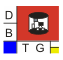
\includegraphics[height=1.5cm]{dbtgBW}};
  \end{tikzpicture}
}
 
\newtheorem{definition}{Definition}
\newtheorem{example}{Example}
\newtheorem{theorem}{Theorem}
\newtheorem{lemma}{Lemma}
\newcommand{\comment}[1]{}
\begin{document}

\begingroup
\let\newpage\relax%
\maketitle
\newpage\null\thispagestyle{blank}\newpage
\setcounter{page}{0}
\endgroup

\begin{abstract}
In this report, we 
\end{abstract}

\tableofcontents

\chapter{Introduction}

Over the years, indexes have been widely used in databases to improve the speed of data retrieval. In the past decades, the database indexes generally fall into hand-engineered data structures and algorithms, such as B-Tree, KD-Tree, Hash Table, etc. These indexes have played an important role in databases and have been widely used in modern data management systems (DBMS). Despite their success, they do not consider the distribution of the database entries, which might be helpful in designing faster indexes.

For example, if the dataset contains integers from $1$ to $1$ million, the key can be used directly as an offset. With the key used as an offset, the values with the key can be retrieved in $\mathcal{O}(1)$ time complexity. Compared with B-Tree, which always takes $\mathcal{O}(\log n)$ time complexity for the same query. At the same time, by using the key as an offset directly, we do not need any extra overhead regarding memory space, where the B-Tree needs extra $\mathcal{O}(n)$ space complexity to save the tree.

From the above example, we found there are two promising advantages of learned indexes over hand-engineered indexes:
\begin{enumerate}
  \item Learned indexes may be faster when performing queries, especially when the number of entries in the database are extremely huge.
  \item Learned indexes may take less memory space, as we only need to save the model with constant size.
  \end{enumerate}
  
 We will explore and analyse these two advantages qualitatively in the \textit{chapter 5}. 

Nowadays, to leverage these two advantages, researchers proposed learned indexes \cite{kraska2018case}, where machine learning techniques are applied to automatically learn the distribution of the database entries and build the data-driven indexes. This approach has been shown to be powerful and competitive compared with hand-engineered indexes, such as B-Tree.

In this report, we explore the development of database indexes, from hand-engineered indexes to the learned index. After that, we explore the possibilities of using complex convolutional neural networks as database indexes. This report is organised into the following chapters:

\begin{enumerate}
	\item \textbf{Introduction}. In this chapter, we illustrate the organisation of this report. Besides, we go through the modern computer systems and introduce the general information about database indexes.
	\item \textbf{Implementation}. In this chapter, we thoroughly describe the implementation of one and two dimensional indexes, including B-Tree, baseline learned index, recursive model, KD-Tree and LISA.
	\item \textbf{Evaluation}. In this chapter, we perform evaluation among the indexes we implemented with different evaluation dataset. 
	\item \textbf{Insights and Findings}. We demonstrate our findings during the implementation in this chapter. Besides, we also discuss the advantages and disadvantages of different indexes.
	\item \textbf{Conclusions}. 
\end{enumerate}

\section{Notations}

In this report, we will use the following notations:

\begin{table}[h]
\begin{tabularx}{\textwidth}{@{}XX@{}}
\toprule
  \underline{Sets and Spaces} \\
  $\mathbb{R}$ & The set of real numbers \\
  $\mathbb{R}^d$ & The set of $d$ dimensional real space \\
  \underline{Random Variables} \\
  $\boldsymbol{X}$ & A vector or matrix \\
  $x$ & A single value in $\textbf{X}$ \\
  $(x,y)$ & A tuple contains two values \\	
  \underline{Hyper-Parameters} \\
  N   & A pre-set hyper parameter \\
  \underline{Functions} \\
  $\mathcal{LR}$ & Linear Regression Function\\
  $\mathcal{P}$ & Polynomial Function\\
  $\mathcal{M}$ & Mapping Function\\
  $\mathcal{O}$ & Big-O notation for complexity\\
  $\mathcal{SP}$ & Shard Prediction Function\\
  $\mathcal{Q}$ & Range Query \\
  $\mathcal{K}$ & $K$NN Query \\
  \underline{Others} \\
  $\clubsuit$ & End of Example \\
  $\blacksquare$ & End of Proof \\
\bottomrule
\end{tabularx}
\end{table}


\section{Terminologies}

In the following chapters, we will use the following terminologies

\textbf{Index model} is a function that maps the index of a row of data into the location (e.g. page index) of the data. For example, in one-dimensional case, the index models include B-Tree, Linear Regression models, etc.

\textbf{Key} is a special attribute in the database that could identify a record. In our work, the key could be a scalar in one-dimensional case, or a $(x,y)$ pair in two-dimensional case.

\textbf{Order of a tree} is the maximum number of children that a node can have.

\textbf{Internal node} is any node of a tree that has child nodes and is not a root node.

\textbf{Leaf node} is any node that does not have child nodes.

\textbf{Level} of a node is defined as the number of edges between this node and the root node.


\section{Motivation}

In traditional database indexes, the complexity for locating an item is usually bounded by some function related to the total number of elements. For example, with a B-Tree, an item can be found within $\mathcal{O}(\log n)$ time complexity. In the meantime, saving a B-Tree as index takes $n$ space complexity. With the rapid growing of the volume of data, $n$ becomes much larger than ever before. Hence, the big data era is calling for a database index that have constant complexity in both time and space.

To achieve such a goal, the distribution of the data is important. For example, assume that the data is fixed-length records over a set of continuous integers from 1 to 100 million, the conventional B-Tree index can be replaced by the keys themselves, making the query time complexity an $\mathcal{O}(1)$ rather than $\mathcal{O}(\log n)$. Similarly, the space complexity would be reduced from $\mathcal{O}(n)$ to $\mathcal{O}(1)$. This example shows that with the knowledge of the distribution of the data, it is possible to locate the item in database in constant time.

Formally, we define the index of each record as $x$ and the corresponding location as $y$ and we represent the whole data as $(X, Y)$ pairs with the total number of pairs defined as $N$. We could then normalise the $Y$ into $\tilde{Y}\in[0,1]$ so that the $\tilde{y}$ represents the portion of the $y$ among the whole $Y$. With these definitions, we can then define a function $F:X\to \tilde{Y}$ that maps the index into the portion of the $y$. We have $y=F(x)* N$. As the output of this function can be considered as the probability of $X\leq x$, we can regard this function $F(x)$ as the cumulative distribution function (CDF) of $X$, i.e. $F(x)=\mathbb{P}(X\leq x)$. Now that $N$ is determined by the length of data records, we only need to learn such CDF and we called the learned CDF function as \textbf{learned index model}.

From the perspective of the distribution of data records, our previous example can be rephrased as following. Our data records are $(X, Y)$ pairs with a linear relation, i.e. $y=x, \forall y\in Y$. We are looking for a function $F$ such that $y=x=F(x)* N$, and hence we end up with $F(x)=\frac{1}{N}*x$. If we use this linear function $F(x)$ as the index model, then we could locate the data within $\mathcal{O}(1)$ time complexity and we only need to store the total number of records as the only parameter. Compared with B-Tree and other indexes, the advantages are enormous.

Even though there might be potential advantages, the learned index model has several assumptions, as listed below.
\begin{enumerate}
	\item All data records are stored in memory. 
	\item All data records are sorted by $X$.
	\item All data records are stored statically in database, hence we do not take insertion and deletion into consideration.
\end{enumerate}




\chapter{Implementation}

\section{One Dimensional Data}

\subsection{B-Tree}

B-tree and its variants have been widely used as indexes in databases. B-trees can be considered as a generalisation of binary search tree: In binary search tree, there is only one key and two children at most in the internal node. B-tree extends the nodes such that each node can contain several keys and children. The keys in a node serve as dividing points and separate the range of keys. With this structure, we make a multi-way decision based on comparisons with the keys stored at the node $x$.

In this section, we introduce the construction process of B-trees and then analyse its properties.

\subsubsection{Attributes and Properties}

Each node \texttt{x} in a B-tree has the following attributes:

\begin{itemize}
\item \texttt{x.n}: the number of keys currently stored in the node $x$.
\item \texttt{x.keys}: the stored keys of this node.
\item \texttt{x.leaf}: a bool value that determines if current node is a leaf node.
\item \texttt{x.children}: a list of its children. If \texttt{x} is a leaf node who has no children at all, then the list will be empty. We assume the children are \texttt{x.$c_1$,$\cdots$,x.$c_{x.n+1}$}, i.e. there will be $\texttt{x.n}+1$ children at most.
\end{itemize}

\noindent
With these attributes, a B-tree has the following properties:

\begin{itemize}
\item The number of children of a node is always $1$ bigger than the number of keys in a node.
\item Nodes in this tree have lower and upper bounds on the number of keys they can contain. These two bounds can be expressed in terms of a fixed integer $t$, which we call the \textbf{minimum degree} of this tree.
	\begin{enumerate}
		\item Each node, other than the root node, must contain at least $t-1$ keys. The root of the tree must have at least one key if the tree is not empty.
		\item Each node can contain at most $2t-1$ keys. A node is called \textbf{full} if it contains exactly $2t-1$ keys.
	\end{enumerate}
\item Inside each node, the keys are sorted in the non-decreasing order, so that we have \texttt{x.keys$_1\leq $} \texttt{x.keys$_2\leq \cdots \leq$} \texttt{x.keys$_{\texttt{x.n}}$}.
\item The keys \texttt{x.key$_i$} separate the ranges of keys stored in each subtree: if $k_i$ is any key stored in the subtree with a root \texttt{x.c$_i$}, then we have $k_1\leq$\texttt{x.keys$_1\leq $}$ k_2\leq$\texttt{x.keys$_2\leq $} $\cdots\leq$ \texttt{x.keys$_n\leq $}$k_{\texttt{x.n}+1}$.
\end{itemize}

In Fig. \ref{fig: B-tree}, we demonstrate an example B-tree whose minimum degree is $2$. In the following section, we will illustrate how to construct and insert keys into a B-tree.

\begin{figure}
\centering
B-tree and its variants have been widely used as indexes in databases. B-trees can be considered as a generalisation of binary search tree: In binary search tree, there is only one key and two children at most in the internal node. B-tree extends the nodes such that each node can contain several keys and children. The keys in a node serve as dividing points and separate the range of keys. With this structure, we make a multi-way decision based on comparisons with the keys stored at the node $x$.

In this section, we introduce the construction process of B-trees and then analyse its properties.

\subsubsection{Attributes and Properties}

Each node \texttt{x} in a B-tree has the following attributes:

\begin{itemize}
\item \texttt{x.n}: the number of keys currently stored in the node $x$.
\item \texttt{x.keys}: the stored keys of this node.
\item \texttt{x.leaf}: a bool value that determines if current node is a leaf node.
\item \texttt{x.children}: a list of its children. If \texttt{x} is a leaf node who has no children at all, then the list will be empty. We assume the children are \texttt{x.$c_1$,$\cdots$,x.$c_{x.n+1}$}, i.e. there will be $\texttt{x.n}+1$ children at most.
\end{itemize}

\noindent
With these attributes, a B-tree has the following properties:

\begin{itemize}
\item The number of children of a node is always $1$ bigger than the number of keys in a node.
\item Nodes in this tree have lower and upper bounds on the number of keys they can contain. These two bounds can be expressed in terms of a fixed integer $t$, which we call the \textbf{minimum degree} of this tree.
	\begin{enumerate}
		\item Each node, other than the root node, must contain at least $t-1$ keys. The root of the tree must have at least one key if the tree is not empty.
		\item Each node can contain at most $2t-1$ keys. A node is called \textbf{full} if it contains exactly $2t-1$ keys.
	\end{enumerate}
\item Inside each node, the keys are sorted in the non-decreasing order, so that we have \texttt{x.keys$_1\leq $} \texttt{x.keys$_2\leq \cdots \leq$} \texttt{x.keys$_{\texttt{x.n}}$}.
\item The keys \texttt{x.key$_i$} separate the ranges of keys stored in each subtree: if $k_i$ is any key stored in the subtree with a root \texttt{x.c$_i$}, then we have $k_1\leq$\texttt{x.keys$_1\leq $}$ k_2\leq$\texttt{x.keys$_2\leq $} $\cdots\leq$ \texttt{x.keys$_n\leq $}$k_{\texttt{x.n}+1}$.
\end{itemize}

In Fig. \ref{fig: B-tree}, we demonstrate an example B-tree whose minimum degree is $2$. In the following section, we will illustrate how to construct and insert keys into a B-tree.

\begin{figure}
\centering
B-tree and its variants have been widely used as indexes in databases. B-trees can be considered as a generalisation of binary search tree: In binary search tree, there is only one key and two children at most in the internal node. B-tree extends the nodes such that each node can contain several keys and children. The keys in a node serve as dividing points and separate the range of keys. With this structure, we make a multi-way decision based on comparisons with the keys stored at the node $x$.

In this section, we introduce the construction process of B-trees and then analyse its properties.

\subsubsection{Attributes and Properties}

Each node \texttt{x} in a B-tree has the following attributes:

\begin{itemize}
\item \texttt{x.n}: the number of keys currently stored in the node $x$.
\item \texttt{x.keys}: the stored keys of this node.
\item \texttt{x.leaf}: a bool value that determines if current node is a leaf node.
\item \texttt{x.children}: a list of its children. If \texttt{x} is a leaf node who has no children at all, then the list will be empty. We assume the children are \texttt{x.$c_1$,$\cdots$,x.$c_{x.n+1}$}, i.e. there will be $\texttt{x.n}+1$ children at most.
\end{itemize}

\noindent
With these attributes, a B-tree has the following properties:

\begin{itemize}
\item The number of children of a node is always $1$ bigger than the number of keys in a node.
\item Nodes in this tree have lower and upper bounds on the number of keys they can contain. These two bounds can be expressed in terms of a fixed integer $t$, which we call the \textbf{minimum degree} of this tree.
	\begin{enumerate}
		\item Each node, other than the root node, must contain at least $t-1$ keys. The root of the tree must have at least one key if the tree is not empty.
		\item Each node can contain at most $2t-1$ keys. A node is called \textbf{full} if it contains exactly $2t-1$ keys.
	\end{enumerate}
\item Inside each node, the keys are sorted in the non-decreasing order, so that we have \texttt{x.keys$_1\leq $} \texttt{x.keys$_2\leq \cdots \leq$} \texttt{x.keys$_{\texttt{x.n}}$}.
\item The keys \texttt{x.key$_i$} separate the ranges of keys stored in each subtree: if $k_i$ is any key stored in the subtree with a root \texttt{x.c$_i$}, then we have $k_1\leq$\texttt{x.keys$_1\leq $}$ k_2\leq$\texttt{x.keys$_2\leq $} $\cdots\leq$ \texttt{x.keys$_n\leq $}$k_{\texttt{x.n}+1}$.
\end{itemize}

In Fig. \ref{fig: B-tree}, we demonstrate an example B-tree whose minimum degree is $2$. In the following section, we will illustrate how to construct and insert keys into a B-tree.

\begin{figure}
\centering
\input{graphs/implementation/one-dim/b-tree}
\caption{An example of B-tree with the minimum degree $t=2$.}
\label{fig: B-tree}
\end{figure}

\subsubsection{Insertion in a B-tree}

With a B-tree, we cannot simply create a new leaf node and insert the new key as we do with a binary search tree, because the resulting tree will fail to be a valid B-tree. Instead, we need to insert the new key into an existing leaf node. If the node is not full, we can safely insert the new key. Otherwise, we will need to split the node around the median of its keys into two new nodes and promote the median key into its parent. In this process, we need to split the parent if its parent is also full.

In the insertion, we travel down the tree and search for the position where the key should be inserted. During the traverse, we split each full node along the way. By doing so, whenever we want to split a full node, we are assured that its parent is not full. The overall algorithm is shown in Algo. \ref{algo:b-tree-insertion}, which contains methods \texttt{splitChild} and \texttt{InsertNonFull} as described in Algo. \ref{algo:b-tree-split-child} and Algo. \ref{algo:b-tree-insert-nonfull} respectively.

\begin{algorithm}[H]
\SetAlgoLined
\SetKwInOut{Input}{input}
\Input{\texttt{T}: The tree with the root \texttt{T.root}; \texttt{k}: The key to be inserted}
\KwResult{\texttt{T}: The tree with the inserted key \texttt{k}}
	\texttt{r=T.root} \\
 \uIf{\texttt{T.n==2t-1}} {
  \texttt{s = NewNode()} \\
  \texttt{T.root = s} \\
  \texttt{s.leaf = False} \\
  \texttt{s.n = 0} \\
  \texttt{s.c$_1$ = r} \\
  \texttt{SplitChild(s, 1)} \\
  \texttt{InsertNonFull(s, k)} \\
 }\uElse{
   \texttt{InsertNonFull(r, k)}
  }
 \caption{Insert}
 \label{algo:b-tree-insertion}
\end{algorithm}

In the Algo. \ref{algo:b-tree-insertion}, we first check if the root node \texttt{r} is full. If it is full, then the root splits and a new node \texttt{s} becomes the root. Then we insert the key \texttt{k} into the tree rooted at the non-full root node, i.e. \texttt{s} or \texttt{r}.

In the Algo. \ref{algo:b-tree-split-child}, the node \texttt{y} originally has $2t$ children (i.e. $2t-1$ keys) and is full. We take the following steps to split it:

\begin{enumerate}
	\item We first (from Line $1$ to Line $11$) create a new node \texttt{z} and give it the largest $t-1$ keys and the corresponding $t$ children of \texttt{y}.
	\item Then we adjust the count of keys for \texttt{y} on Line $12$: after the split, \texttt{y} will have $t-1$ keys.
	\item After that, from Line $13$ to Line $21$, we insert \texttt{z} as a child of \texttt{x}, move the median key from \texttt{y} up to \texttt{x}, and adjust the key count in \texttt{x}.
\end{enumerate}

\begin{algorithm}[H]
\SetAlgoLined
\SetKwInOut{Input}{input}
\Input{\texttt{x}: The node whose children are being split; \texttt{i}: The index of \texttt{x}'s child who is full originally}
\KwResult{\texttt{x}: The parent node whose children are not full}
\texttt{z = NewNode()} \\
\texttt{y = x.c$_i$}  \\
\texttt{z.leaf = y.leaf} \\
\texttt{z.n = t-1}\\
\For{$j\gets1$ \KwTo $t-1$}{
  \texttt{z.keys$_j$ = y.keys$_{j+t}$}\\
}
\uIf{not \texttt{y.leaf}} {
	\For{$j\gets 1$\KwTo $t$} {
		\texttt{z.c$_j$ = y.c$_{j+t}$} \\
	}
}
\texttt{y.n = t-1}\\
\For{$j\gets \texttt{x.n}$ \KwTo $i+1$} {
	\texttt{x.c$_{j+1}$ = x.c$_j$}
}
\texttt{x.c$_{i+1}$ = z} \\
\For{$j\gets \texttt{x.n}$ \KwTo $i$} {
	\texttt{x.keys$_{j+1}$=x.keys$_j$}
}
\texttt{x.key$_i$ = y.key$_t$}\\
\texttt{x.n = x.n+1}
\caption{SplitChild}
\label{algo:b-tree-split-child}	
\end{algorithm}

The Algo. \ref{algo:b-tree-insert-nonfull} works as follows:

\begin{enumerate}
	\item From Line $3$ to Line $6$, We first check if \texttt{x} is a leaf. If it is a leaf, then we insert the key \texttt{k} into \texttt{x}.
	\item If \texttt{x} is not a leaf, then we must insert \texttt{k} into the appropriate leaf node in the subtree rooted at internal node \texttt{x}. From Line $8$ to Line $11$, we traverse the subtree rooted at \texttt{x} and determine the child of \texttt{x} to which the recursion descends. Then we check on Line $12$ if the child where the recursion descends is a full node.
	\item If the child is a full node, we then split the child on Line $13$ into two non-full children. We then determine from Line $14$ to Line $15$ which of the two children is the appropriate node to insert.
	\item At the last, on Line $16$ we look into the $i$th children of \texttt{x} and recursively insert the key \texttt{k} into it.
\end{enumerate}

\begin{algorithm}[H]
\SetAlgoLined
\SetKwInOut{Input}{input}
\Input{\texttt{x}: The node to be inserted; \texttt{k}: The key to be inserted}
\KwResult{\texttt{x}: The node with the inserted key \texttt{k}}
\texttt{i=x.n} \\
\uIf{\texttt{x.leaf}} {
	\While{\texttt{i $\geq$ 1 and k < x.keys$_i$}} {
		\texttt{x.key$_{i+1}$=k} \\
		\texttt{x.n = x.n+1} \\
	}
}
\uElse{
	\While{\texttt{i $\geq$ 1 and k < x.keys$_i$}} {
		\texttt{i=i-1}\\
	}
	\texttt{i=i+1} \\
	\uIf{\texttt{x.c$_i$.n==2t-1}} {
		\texttt{SplitChild(x,i)} \\
		\uIf{\texttt{k>x.key$_i$}} {
			\texttt{i=i+1} \\
		}
	}
	\texttt{InsertNonFull(x.c$_i$, k)}
}
\caption{InsertNonFull}
\label{algo:b-tree-insert-nonfull}	
\end{algorithm}

\caption{An example of B-tree with the minimum degree $t=2$.}
\label{fig: B-tree}
\end{figure}

\subsubsection{Insertion in a B-tree}

With a B-tree, we cannot simply create a new leaf node and insert the new key as we do with a binary search tree, because the resulting tree will fail to be a valid B-tree. Instead, we need to insert the new key into an existing leaf node. If the node is not full, we can safely insert the new key. Otherwise, we will need to split the node around the median of its keys into two new nodes and promote the median key into its parent. In this process, we need to split the parent if its parent is also full.

In the insertion, we travel down the tree and search for the position where the key should be inserted. During the traverse, we split each full node along the way. By doing so, whenever we want to split a full node, we are assured that its parent is not full. The overall algorithm is shown in Algo. \ref{algo:b-tree-insertion}, which contains methods \texttt{splitChild} and \texttt{InsertNonFull} as described in Algo. \ref{algo:b-tree-split-child} and Algo. \ref{algo:b-tree-insert-nonfull} respectively.

\begin{algorithm}[H]
\SetAlgoLined
\SetKwInOut{Input}{input}
\Input{\texttt{T}: The tree with the root \texttt{T.root}; \texttt{k}: The key to be inserted}
\KwResult{\texttt{T}: The tree with the inserted key \texttt{k}}
	\texttt{r=T.root} \\
 \uIf{\texttt{T.n==2t-1}} {
  \texttt{s = NewNode()} \\
  \texttt{T.root = s} \\
  \texttt{s.leaf = False} \\
  \texttt{s.n = 0} \\
  \texttt{s.c$_1$ = r} \\
  \texttt{SplitChild(s, 1)} \\
  \texttt{InsertNonFull(s, k)} \\
 }\uElse{
   \texttt{InsertNonFull(r, k)}
  }
 \caption{Insert}
 \label{algo:b-tree-insertion}
\end{algorithm}

In the Algo. \ref{algo:b-tree-insertion}, we first check if the root node \texttt{r} is full. If it is full, then the root splits and a new node \texttt{s} becomes the root. Then we insert the key \texttt{k} into the tree rooted at the non-full root node, i.e. \texttt{s} or \texttt{r}.

In the Algo. \ref{algo:b-tree-split-child}, the node \texttt{y} originally has $2t$ children (i.e. $2t-1$ keys) and is full. We take the following steps to split it:

\begin{enumerate}
	\item We first (from Line $1$ to Line $11$) create a new node \texttt{z} and give it the largest $t-1$ keys and the corresponding $t$ children of \texttt{y}.
	\item Then we adjust the count of keys for \texttt{y} on Line $12$: after the split, \texttt{y} will have $t-1$ keys.
	\item After that, from Line $13$ to Line $21$, we insert \texttt{z} as a child of \texttt{x}, move the median key from \texttt{y} up to \texttt{x}, and adjust the key count in \texttt{x}.
\end{enumerate}

\begin{algorithm}[H]
\SetAlgoLined
\SetKwInOut{Input}{input}
\Input{\texttt{x}: The node whose children are being split; \texttt{i}: The index of \texttt{x}'s child who is full originally}
\KwResult{\texttt{x}: The parent node whose children are not full}
\texttt{z = NewNode()} \\
\texttt{y = x.c$_i$}  \\
\texttt{z.leaf = y.leaf} \\
\texttt{z.n = t-1}\\
\For{$j\gets1$ \KwTo $t-1$}{
  \texttt{z.keys$_j$ = y.keys$_{j+t}$}\\
}
\uIf{not \texttt{y.leaf}} {
	\For{$j\gets 1$\KwTo $t$} {
		\texttt{z.c$_j$ = y.c$_{j+t}$} \\
	}
}
\texttt{y.n = t-1}\\
\For{$j\gets \texttt{x.n}$ \KwTo $i+1$} {
	\texttt{x.c$_{j+1}$ = x.c$_j$}
}
\texttt{x.c$_{i+1}$ = z} \\
\For{$j\gets \texttt{x.n}$ \KwTo $i$} {
	\texttt{x.keys$_{j+1}$=x.keys$_j$}
}
\texttt{x.key$_i$ = y.key$_t$}\\
\texttt{x.n = x.n+1}
\caption{SplitChild}
\label{algo:b-tree-split-child}	
\end{algorithm}

The Algo. \ref{algo:b-tree-insert-nonfull} works as follows:

\begin{enumerate}
	\item From Line $3$ to Line $6$, We first check if \texttt{x} is a leaf. If it is a leaf, then we insert the key \texttt{k} into \texttt{x}.
	\item If \texttt{x} is not a leaf, then we must insert \texttt{k} into the appropriate leaf node in the subtree rooted at internal node \texttt{x}. From Line $8$ to Line $11$, we traverse the subtree rooted at \texttt{x} and determine the child of \texttt{x} to which the recursion descends. Then we check on Line $12$ if the child where the recursion descends is a full node.
	\item If the child is a full node, we then split the child on Line $13$ into two non-full children. We then determine from Line $14$ to Line $15$ which of the two children is the appropriate node to insert.
	\item At the last, on Line $16$ we look into the $i$th children of \texttt{x} and recursively insert the key \texttt{k} into it.
\end{enumerate}

\begin{algorithm}[H]
\SetAlgoLined
\SetKwInOut{Input}{input}
\Input{\texttt{x}: The node to be inserted; \texttt{k}: The key to be inserted}
\KwResult{\texttt{x}: The node with the inserted key \texttt{k}}
\texttt{i=x.n} \\
\uIf{\texttt{x.leaf}} {
	\While{\texttt{i $\geq$ 1 and k < x.keys$_i$}} {
		\texttt{x.key$_{i+1}$=k} \\
		\texttt{x.n = x.n+1} \\
	}
}
\uElse{
	\While{\texttt{i $\geq$ 1 and k < x.keys$_i$}} {
		\texttt{i=i-1}\\
	}
	\texttt{i=i+1} \\
	\uIf{\texttt{x.c$_i$.n==2t-1}} {
		\texttt{SplitChild(x,i)} \\
		\uIf{\texttt{k>x.key$_i$}} {
			\texttt{i=i+1} \\
		}
	}
	\texttt{InsertNonFull(x.c$_i$, k)}
}
\caption{InsertNonFull}
\label{algo:b-tree-insert-nonfull}	
\end{algorithm}

\caption{An example of B-tree with the minimum degree $t=2$.}
\label{fig: B-tree}
\end{figure}

\subsubsection{Insertion in a B-tree}

With a B-tree, we cannot simply create a new leaf node and insert the new key as we do with a binary search tree, because the resulting tree will fail to be a valid B-tree. Instead, we need to insert the new key into an existing leaf node. If the node is not full, we can safely insert the new key. Otherwise, we will need to split the node around the median of its keys into two new nodes and promote the median key into its parent. In this process, we need to split the parent if its parent is also full.

In the insertion, we travel down the tree and search for the position where the key should be inserted. During the traverse, we split each full node along the way. By doing so, whenever we want to split a full node, we are assured that its parent is not full. The overall algorithm is shown in Algo. \ref{algo:b-tree-insertion}, which contains methods \texttt{splitChild} and \texttt{InsertNonFull} as described in Algo. \ref{algo:b-tree-split-child} and Algo. \ref{algo:b-tree-insert-nonfull} respectively.

\begin{algorithm}[H]
\SetAlgoLined
\SetKwInOut{Input}{input}
\Input{\texttt{T}: The tree with the root \texttt{T.root}; \texttt{k}: The key to be inserted}
\KwResult{\texttt{T}: The tree with the inserted key \texttt{k}}
	\texttt{r=T.root} \\
 \uIf{\texttt{T.n==2t-1}} {
  \texttt{s = NewNode()} \\
  \texttt{T.root = s} \\
  \texttt{s.leaf = False} \\
  \texttt{s.n = 0} \\
  \texttt{s.c$_1$ = r} \\
  \texttt{SplitChild(s, 1)} \\
  \texttt{InsertNonFull(s, k)} \\
 }\uElse{
   \texttt{InsertNonFull(r, k)}
  }
 \caption{Insert}
 \label{algo:b-tree-insertion}
\end{algorithm}

In the Algo. \ref{algo:b-tree-insertion}, we first check if the root node \texttt{r} is full. If it is full, then the root splits and a new node \texttt{s} becomes the root. Then we insert the key \texttt{k} into the tree rooted at the non-full root node, i.e. \texttt{s} or \texttt{r}.

In the Algo. \ref{algo:b-tree-split-child}, the node \texttt{y} originally has $2t$ children (i.e. $2t-1$ keys) and is full. We take the following steps to split it:

\begin{enumerate}
	\item We first (from Line $1$ to Line $11$) create a new node \texttt{z} and give it the largest $t-1$ keys and the corresponding $t$ children of \texttt{y}.
	\item Then we adjust the count of keys for \texttt{y} on Line $12$: after the split, \texttt{y} will have $t-1$ keys.
	\item After that, from Line $13$ to Line $21$, we insert \texttt{z} as a child of \texttt{x}, move the median key from \texttt{y} up to \texttt{x}, and adjust the key count in \texttt{x}.
\end{enumerate}

\begin{algorithm}[H]
\SetAlgoLined
\SetKwInOut{Input}{input}
\Input{\texttt{x}: The node whose children are being split; \texttt{i}: The index of \texttt{x}'s child who is full originally}
\KwResult{\texttt{x}: The parent node whose children are not full}
\texttt{z = NewNode()} \\
\texttt{y = x.c$_i$}  \\
\texttt{z.leaf = y.leaf} \\
\texttt{z.n = t-1}\\
\For{$j\gets1$ \KwTo $t-1$}{
  \texttt{z.keys$_j$ = y.keys$_{j+t}$}\\
}
\uIf{not \texttt{y.leaf}} {
	\For{$j\gets 1$\KwTo $t$} {
		\texttt{z.c$_j$ = y.c$_{j+t}$} \\
	}
}
\texttt{y.n = t-1}\\
\For{$j\gets \texttt{x.n}$ \KwTo $i+1$} {
	\texttt{x.c$_{j+1}$ = x.c$_j$}
}
\texttt{x.c$_{i+1}$ = z} \\
\For{$j\gets \texttt{x.n}$ \KwTo $i$} {
	\texttt{x.keys$_{j+1}$=x.keys$_j$}
}
\texttt{x.key$_i$ = y.key$_t$}\\
\texttt{x.n = x.n+1}
\caption{SplitChild}
\label{algo:b-tree-split-child}	
\end{algorithm}

The Algo. \ref{algo:b-tree-insert-nonfull} works as follows:

\begin{enumerate}
	\item From Line $3$ to Line $6$, We first check if \texttt{x} is a leaf. If it is a leaf, then we insert the key \texttt{k} into \texttt{x}.
	\item If \texttt{x} is not a leaf, then we must insert \texttt{k} into the appropriate leaf node in the subtree rooted at internal node \texttt{x}. From Line $8$ to Line $11$, we traverse the subtree rooted at \texttt{x} and determine the child of \texttt{x} to which the recursion descends. Then we check on Line $12$ if the child where the recursion descends is a full node.
	\item If the child is a full node, we then split the child on Line $13$ into two non-full children. We then determine from Line $14$ to Line $15$ which of the two children is the appropriate node to insert.
	\item At the last, on Line $16$ we look into the $i$th children of \texttt{x} and recursively insert the key \texttt{k} into it.
\end{enumerate}

\begin{algorithm}[H]
\SetAlgoLined
\SetKwInOut{Input}{input}
\Input{\texttt{x}: The node to be inserted; \texttt{k}: The key to be inserted}
\KwResult{\texttt{x}: The node with the inserted key \texttt{k}}
\texttt{i=x.n} \\
\uIf{\texttt{x.leaf}} {
	\While{\texttt{i $\geq$ 1 and k < x.keys$_i$}} {
		\texttt{x.key$_{i+1}$=k} \\
		\texttt{x.n = x.n+1} \\
	}
}
\uElse{
	\While{\texttt{i $\geq$ 1 and k < x.keys$_i$}} {
		\texttt{i=i-1}\\
	}
	\texttt{i=i+1} \\
	\uIf{\texttt{x.c$_i$.n==2t-1}} {
		\texttt{SplitChild(x,i)} \\
		\uIf{\texttt{k>x.key$_i$}} {
			\texttt{i=i+1} \\
		}
	}
	\texttt{InsertNonFull(x.c$_i$, k)}
}
\caption{InsertNonFull}
\label{algo:b-tree-insert-nonfull}	
\end{algorithm}


\subsection{Baseline Learned Index}

\subsubsection{Overview}

The B-Tree can be regarded as a function $\mathcal{F}$ that maps the key $x$ into its corresponding page index $y$. It is known to us that the pages are allocated in a way that the every $S$ entries are allocated in a page where $S$ is a pre-defined parameter. For example, if we set $S$ to be 10 items per page, then the first page will contain the first 10 keys and their corresponding values. Similarly, the second 10 keys and their corresponding values will be allocated to the second page.

If we know the CDF of $X$ as $F(X\leq x)$ and the total number of entries $N$, then the position of $x$ can be estimated as $p=F(x)*N$ and the page index where it should be allocated to is given by

$$y=\floor{\frac{p}{S}}=\floor{\frac{F(x)*N}{S}}$$  

For example, if the keys are uniformly distributed from $0$ to $1000$, i.e. the CDF of $X$ is defined as $F(X\leq x)=\frac{x}{1000}$ and we set $S=10, N=1001$. Then for any key $x$, we immediately know it will be allocated into $y=\floor{\frac{1000}{10}*\frac{x}{1000}}=\floor{\frac{x}{10}}$. Assume that we have a key $698$, then we can calculate $y=\floor{\frac{698}{10}}=69$. By doing so, the page index is calculated in constant time and space.

In this example, we see that the distribution of $X$ is essential and our goal of learned index in one-dimensional data is to learn such distribution. To do so, we apply two different techniques as the baseline, the polynomial regression and fully connected neural network.

To train such a learned index, we first manually generate the $X$ with respect to a certain distribution. We then save the generated $X$ into a dense array with the length $N$. Then we use the proportional index, i.e. the index of each $x$ divided by $N$ as the expected output $y$.

\subsubsection{Polynomial Regression}
 
The polynomial regression model with degree $m$ can be formalised as 

$$ \hat{y_i}= \beta_0+\beta_1x_i+\beta_2x_i^2+\cdots+\beta_mx_i^m$$ and it can be expressed in a matrix form as below

$$
\begin{bmatrix}
y_1 \\ y_2\\ \vdots \\ y_n 
\end{bmatrix}=\begin{bmatrix}
1 & x_1 & x_1^2 &\cdots & x_1^m \\ 
1 & x_2 & x_2^2 &\cdots & x_2^m \\ 
\vdots \\ 
1 & x_n & x_n^2 &\cdots & x_n^m \\ 
\end{bmatrix}\begin{bmatrix}
\beta_0 \\ \beta_1 \\ \vdots \\ \beta_m 
\end{bmatrix}
$$ which can be written as $Y=\boldsymbol{X}\boldsymbol{\beta}$. 
 
 Our goal is to find $\beta$ such that the sum of squared error, i.e. $\text{S}(\boldsymbol{\beta})=\sum_{i=1}^n(\hat{y}-y)^2$ is minimal. This optimisation problem can be resolved by ordinary least square estimation as shown below.
 
 First we have the error as
 
 \begin{equation}
 \begin{split}
 \text{S}(\boldsymbol{\beta})=||\boldsymbol{y}-\boldsymbol{X} \boldsymbol{\beta}||& =(\boldsymbol{y}-\boldsymbol{X}\boldsymbol{\beta})^T(\boldsymbol{y}-\boldsymbol{X}\boldsymbol{\beta})\\
 	& =\boldsymbol{y}^T\boldsymbol{y}-\boldsymbol{\beta}^T\boldsymbol{X}^T\boldsymbol{y}-\boldsymbol{y}^T\boldsymbol{X}\boldsymbol{\beta}+\boldsymbol{\beta}^T\boldsymbol{X}^T\boldsymbol{X}\boldsymbol{\beta}
\end{split}
 \end{equation}
 
 Here we know that $(\boldsymbol{\beta}^T\boldsymbol{X}^T\boldsymbol{y})^T=\boldsymbol{y}^T\boldsymbol{X}\boldsymbol{\beta}$ is a $1\times 1$ matrix, i.e. a scalar. Hence it is equal to its own transpose. As a result we could simplify the error as
 
 \begin{equation}
 	\begin{split}
 		\text{S}(\boldsymbol{\beta})=\boldsymbol{y}^T\boldsymbol{y}-2\boldsymbol{\beta}^T\boldsymbol{X}^T\boldsymbol{y}+\boldsymbol{\beta}^T\boldsymbol{X}^T\boldsymbol{X}\boldsymbol{\beta}
 	\end{split}
 \end{equation}
 
 In order to find the minimum of $S(\boldsymbol{\beta})$, we differentiate it with respect to $\boldsymbol{\beta}$ as 
 
 \begin{equation}
 	\nabla_{\boldsymbol{\beta}}S=-2\boldsymbol{X}^T\boldsymbol{y}+2(\boldsymbol{X}^T\boldsymbol{X})\boldsymbol{\beta}
 \end{equation}
 
 By let it to be zero, we end up with 
 
 \begin{equation}
 \begin{split}
 	 &	-\boldsymbol{X}^T\boldsymbol{y}+(\boldsymbol{X}^T\boldsymbol{X})\boldsymbol{\beta}=0 \\
 	& \implies \boldsymbol{\beta}= (\boldsymbol{X}^T\boldsymbol{X})^{-1}\boldsymbol{X}^T\boldsymbol{y}
 \end{split}
 \end{equation}
 
\subsubsection{Fully Connected Neural Network}

\subsection{Recursive Model Index}

%TODO: there should be some graph to demonstrate the last-mile problem.

In our baseline models, it is not very difficult to reduce the mean square error from millions to thousands. However, it is much harder to reduce it from thousands to tens. This is the so called last-mile problem.

In order to solve this problem, recursive model index was proposed \cite{kraska2018case}. The idea is to split the whole set of data into smaller pieces and assign each piece an index model. By doing so, each model is only responsible for a small range of keys. Ideally, in each smaller range, the keys are distributed in a way that is easier to be learned by our index models, such as polynomial model, fully connected model or even traditional B-Tree model.

As shown in Fig. \ref{rmi_structure}. A recursive model can be regarded as a tree structure, which contains a root model that receives the full dataset for training. Then the root model will split the dataset into several parts. Each sub-model will then receive one part of the full dataset. Then we train the sub-models one by one with the partial training dataset. 

\begin{mscexample}
	For example, in the Fig. \ref{rmi_structure}, the full dataset will be split into three parts and each sub-model receives one part. To train this recursive model, we first train the root model with the whole dataset. Then the root model will split the dataset into 3 parts according to the predicted value of each data point in the dataset. Then each sub-model will receive one part and we train the sub-model accordingly.
\end{mscexample}

\begin{figure*}[h]
\centering
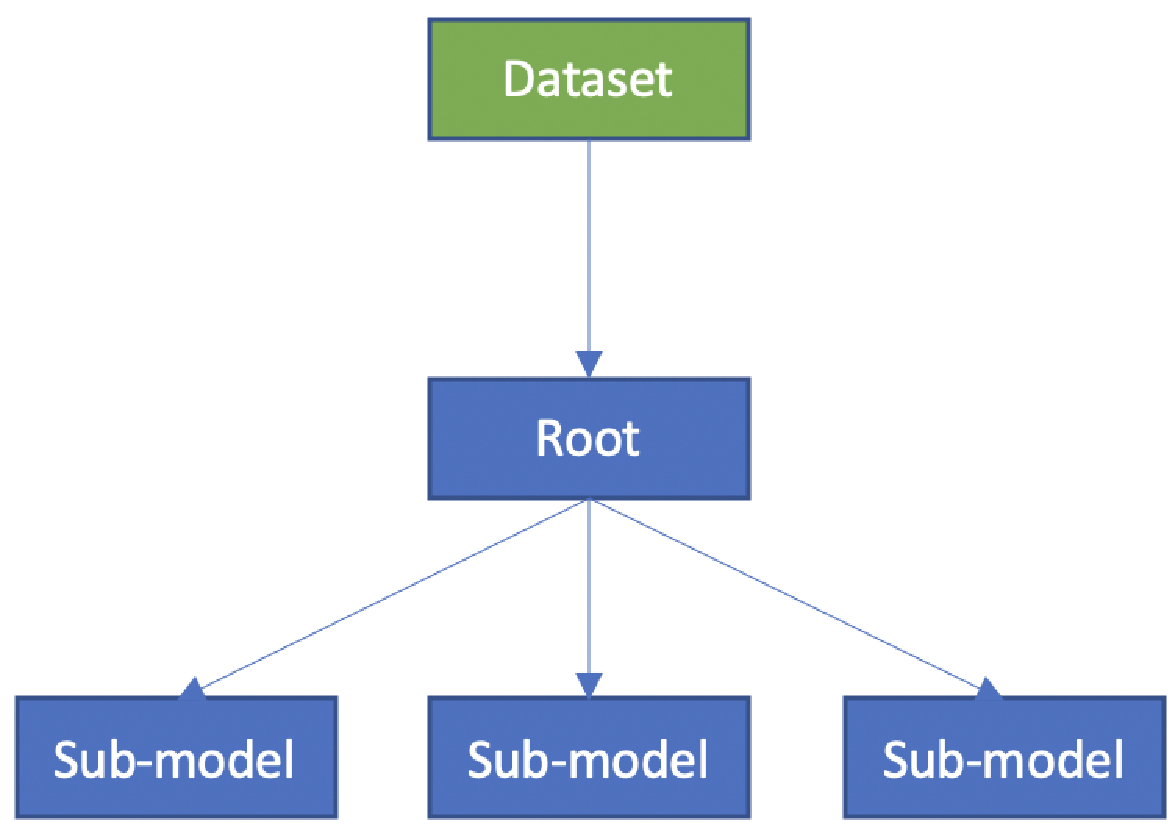
\includegraphics[scale=0.4]{graphs/rmi_demo}
\caption{An example recursive model index with one root model and three leaf model.}
\label{rmi_structure}
\end{figure*}



\subsubsection{Definitions}

Similar to a tree, we define the following terms in a recursive model:

\begin{enumerate}
	\item \textbf{Node Model}. Every node is responsible for making decisions with given input data. In one dimensional case, it can be regarded as a function $f:\mathbb{R}\to\mathbb{R}, x\to y$ where $x$ is the input index and $y$ is the corresponding page block. In principle, each node can be implemented as any machine learning model, from linear regression to neural network, or a traditional tree-based model, such as B-Tree.
	\item \textbf{Internal Node Model}. Internal nodes are all nodes except for leaf nodes and the root node. Every internal node receives a certain part of training data from the full dataset, and train a model on it. 
\end{enumerate}

In the following sections, we will use the notations defined below:
\begin{enumerate}
	\item $N_M^{(i)}$ is the number of models in the $i$th stage.
	%TODO: more notations
	%TODO: modify algorithms accordingly
\end{enumerate}


\subsubsection{Training}

In order to construct a recursive model, we need to have several parameters listed below:
\begin{enumerate}
	\item The training dataset, notated as $(X, Y)$ with entries notated as $(x,y)$.
	\item The number of stages, notated as $N_S$. It is an integer variable.
	\item The number of models at each stage, notated as $N_M$. It is a list of integer variable. $N_M^{(i+1)}$ represents the number of models in the $i$th stage.
\end{enumerate}

The training process of recursive model is an up-bottom process. There will be only one root model that receives the whole training data. After the root model is trained, we iterate over all the training data and predict the page by the root model. After the iteration, we get a new set of pairs $(X, Y_0)$. Then we map $\forall y_0\in Y_0$ into the selected model id in next stage by $\texttt{next}=y_0 * N_M^{(i+1)}/\texttt{max(Y)}$.

\begin{algorithm}[H]
    \SetAlgoLined
    \SetKwInOut{Input}{input}
    \Input{\texttt{num\_of\_stages; num\_of\_models; types\_of\_models; x; y}}
     \texttt{trainset=[[(x,y)]]} \\
     \texttt{stage$\gets 0$} \\
     \While{\texttt{stage} \textless \texttt{num\_of\_stages}}{
      \While{\texttt{model} \textless \texttt{num\_of\_models[stage]}} {
        \texttt{model.train(trainset[stage][model])} \\
        \texttt{models[stage].append(model)}
      }
      \uIf{not last stage} {
        \For{$i\gets0$ \KwTo $len(x)$}{
            	\texttt{model=models[output from previous stage]} \\
            	\texttt{output=model.predict(x[i])} \\
            	\texttt{next=output * num\_of\_models[stage+1]/max\_y} \\
            	\texttt{trainset[stage+1][next].add((x[i],y[i]))}
        }
      }
     }
     \caption{Training of Recursive Model Index}
\end{algorithm}

\subsubsection{Prediction}

\begin{algorithm}[H]
    \SetAlgoLined
    \SetKwInOut{Input}{input}
    \Input{\texttt{x; models; num\_of\_stages; max\_y}}
     \texttt{stage$\gets 0$} \\
 	 \texttt{next\_model$\gets 0$} \\
     \While{\texttt{stage} \textless \texttt{num\_of\_stages}}{
        \texttt{output = model.predict(x)} \\
        \texttt{next\_model=output*len(models[stage+1])/max\_y}\\ 
      \uIf{last stage} {
		\texttt{y = next}
      }
     }
     \caption{Training of Recursive Model Index}
\end{algorithm}

\subsubsection{Polynomial Internal Models}

In the recursive model index, we use internal models to learn the CDF of a part of the full training data. In order to learn the CDF, we need to know or assume the distribution of a specific part of the data. In this report, we support the following distributions.

\begin{table}[h]
  \begin{tabularx}{\textwidth}{@{}XX@{}}
  \toprule
    Linear Regression & $wx+b$ \\
    Quadratic Regression & $ax^2+bx+c$ \\
    B-Tree & N/A \\
    Fully Connected Neural Network & N/A \\
  \bottomrule
  \end{tabularx}
  \end{table}

Here we describe how we fit a polynomial model.

The polynomial regression model with degree $m$ can be formalised as 

$$ \hat{y_i}= \beta_0+\beta_1x_i+\beta_2x_i^2+\cdots+\beta_mx_i^m$$ and it can be expressed in a matrix form as below

$$
\begin{bmatrix}
y_1 \\ y_2\\ \vdots \\ y_n 
\end{bmatrix}=\begin{bmatrix}
1 & x_1 & x_1^2 &\cdots & x_1^m \\ 
1 & x_2 & x_2^2 &\cdots & x_2^m \\ 
\vdots \\ 
1 & x_n & x_n^2 &\cdots & x_n^m \\ 
\end{bmatrix}\begin{bmatrix}
\beta_0 \\ \beta_1 \\ \vdots \\ \beta_m 
\end{bmatrix}
$$ which can be written as $Y=\boldsymbol{X}\boldsymbol{\beta}$. 
 
 Our goal is to find $\beta$ such that the sum of squared error, i.e. $\text{S}(\boldsymbol{\beta})=\sum_{i=1}^n(\hat{y}-y)^2$ is minimal. This optimisation problem can be resolved by ordinary least square estimation as shown below.
 
 First we have the error as
 
 \begin{equation}
 \begin{split}
 \text{S}(\boldsymbol{\beta})=||\boldsymbol{y}-\boldsymbol{X} \boldsymbol{\beta}||& =(\boldsymbol{y}-\boldsymbol{X}\boldsymbol{\beta})^T(\boldsymbol{y}-\boldsymbol{X}\boldsymbol{\beta})\\
 	& =\boldsymbol{y}^T\boldsymbol{y}-\boldsymbol{\beta}^T\boldsymbol{X}^T\boldsymbol{y}-\boldsymbol{y}^T\boldsymbol{X}\boldsymbol{\beta}+\boldsymbol{\beta}^T\boldsymbol{X}^T\boldsymbol{X}\boldsymbol{\beta}
\end{split}
 \end{equation}
 
 Here we know that $(\boldsymbol{\beta}^T\boldsymbol{X}^T\boldsymbol{y})^T=\boldsymbol{y}^T\boldsymbol{X}\boldsymbol{\beta}$ is a $1\times 1$ matrix, i.e. a scalar. Hence it is equal to its own transpose. As a result we could simplify the error as
 
 \begin{equation}
 	\begin{split}
 		\text{S}(\boldsymbol{\beta})=\boldsymbol{y}^T\boldsymbol{y}-2\boldsymbol{\beta}^T\boldsymbol{X}^T\boldsymbol{y}+\boldsymbol{\beta}^T\boldsymbol{X}^T\boldsymbol{X}\boldsymbol{\beta}
 	\end{split}
 \end{equation}
 
 In order to find the minimum of $S(\boldsymbol{\beta})$, we differentiate it with respect to $\boldsymbol{\beta}$ as 
 
 \begin{equation}
 	\nabla_{\boldsymbol{\beta}}S=-2\boldsymbol{X}^T\boldsymbol{y}+2(\boldsymbol{X}^T\boldsymbol{X})\boldsymbol{\beta}
 \end{equation}
 
 By let it to be zero, we end up with 
 
 \begin{equation}
 \begin{split}
 	 &	-\boldsymbol{X}^T\boldsymbol{y}+(\boldsymbol{X}^T\boldsymbol{X})\boldsymbol{\beta}=0 \\
 	& \implies \boldsymbol{\beta}= (\boldsymbol{X}^T\boldsymbol{X})^{-1}\boldsymbol{X}^T\boldsymbol{y}
 \end{split}
 \end{equation}

  

\section{Two Dimensional Data}

\subsection{LISA: Learned Index for Spatial Data}

\comm{
\subsubsection{LISA Baseline model Limitation}

Prediction cost in baseline method consists of following two parts.

\begin{enumerate}
	\item Search cost for the cell which contains the key. This cost will be equal to $log_{2}N_{1}$, where $N_{1}$ is the number of cells into which mapped values are divided.
	
	\item Cost associated with sequentially comparing the query point key value against keys inside the cell found in previous search. On average this cost will be equal to $N_{2}\slash2$, where $N_{2}$ is the number of keys in a cell.   
	
If cell size is large, number of cells will be smaller, number of keys per cell will be higher, resulting in higher cost of sequential scan with in the cell. 
\end{enumerate}
Consider the example in figure \ref{fig:BaseLine_Method_Limitation}. Dataset is divided into 3 sections based on the mapped values. Any point or range query in the second triangle(page) will result into a sequential scan through all 9 keys in the cells.

\begin{figure*}[t]
    \centering
    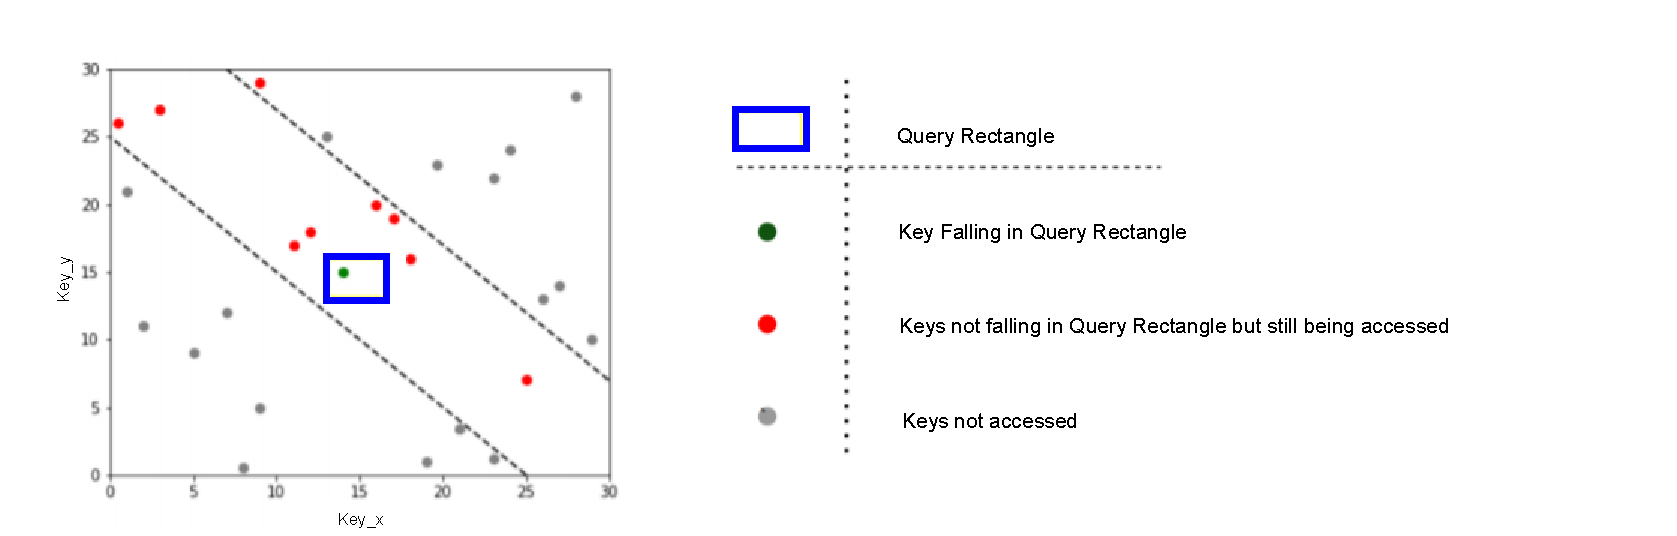
\includegraphics[width=1.3\textwidth]{graphs/Baseline_limitation.pdf}
    \caption{Baseline Method Limitation }
    \label{fig:BaseLine_Method_Limitation}
\end{figure*}
}


\subsubsection {LISA Baseline model search optimization for smaller values of N}
%In lisa baseline model, we need to linearly search for the query key in a cell. 
In case of high dimensional key values, key with in a cell can not be searched with mapped value, as a large number of keys can have the same mapped value. However for the 2 dimensional scenario, we can get considerable savings in search cost by replacing sequential scan based on keys values to binary search based on mapped value. As in the original method, search process  will consist of two parts.
\begin{enumerate}
	\item Find the cell which contains the query key based on mapped value using binary search. 
	\item With in the cell, replace sequential search based on query key value with the  binary search based on query key mapped value. Once mapped value is found, do a lookup in the neighbourhood of the found key based on query key 2 dimensional value. 
\end{enumerate}
As shown in Fig. \ref{fig:LISA_Baseline_Optimization}, we get significant savings in the query time with this approach for smaller values of N. As the value of $N$ increases, number of Keys per cell decreases, and savings in avoiding sequential search gets normalized. 


\begin{figure}
 \centering
     \begin{subfigure}[b]{0.45\textwidth}
         \centering
         \begin{tikzpicture}[font=\small]
	\pgfplotsset{compat=1.10, width=\textwidth, height=\textwidth,every axis
	legend/.append style={
		at={(1,1)},
		anchor=north east}}
	\begin{axis}[
		xmode=log,
		xlabel=$N$,
		ylabel=Average Query Time (ms),
		xtick={10,100,1000,10000},
		legend style={nodes={scale=0.55, transform shape}}
	]
	\addplot[smooth, mark=x, blue]
	coordinates{
		(10, 46.7173)
		(100, 4.8086)
		(1000, 0.7271)
		(10000,0.3301)
		%(100000,0.2381)
	};
	\addplot[smooth,mark=o,red]
  	coordinates{
        (10, 0.2855)
		(100,0.2823)
		(1000, 0.2806)
		(10000,0.2794)
		%(100000,0.2322)
	};
  
    %\legend{LISA Baseline, LISA Baseline Optimized}
	\end{axis}
\end{tikzpicture}
         \caption{Training Size 100K}
         \label{fig:2d_exp4_3_1}
     \end{subfigure}
     \begin{subfigure}[b]{0.45\textwidth}
         \centering
         \begin{tikzpicture}[font=\small]
	\pgfplotsset{compat=1.10, width=\textwidth, height=\textwidth,every axis
	legend/.append style={
		at={(1,1)},
		anchor=north east}}
	\begin{axis}[
		xmode=log,
		xlabel=$N$,
		ylabel=Average Query Time (ms),
		xtick={10,100,1000,10000},
		legend style={nodes={scale=0.75, transform shape}},
		scaled y ticks = base 10:-2,
	]
	\addplot[smooth, mark=x, blue]
	coordinates{
		(10, 347.5613)
		(100, 40.1451)
		(1000, 4.4732)
		(10000,0.6697)
		%(100000,0.2944)
	};
	\addplot[smooth,mark=o,red]
  	coordinates{
        (10, 0.2905)
		(100,0.2858)
		(1000, 0.2844)
		(10000,0.2831)
		%(100000,0.2322)
	};
  
    \legend{LISA Baseline, LISA Baseline Optimized}
	\end{axis}
\end{tikzpicture}
         \caption{Training Size 1M}
         \label{fig:2d_exp4_3_2}
     \end{subfigure}
     \caption{Point query results comparison between LISA Baseline and Optimized Model for different training sizes.}
     \label{fig:LISA_Baseline_Optimization}
\end{figure}



\chapter{Evaluation}

\chapter{Insights and Findings}

\chapter{Conclusion}

\bibliographystyle{alpha}
\bibliography{refs}

\end{document}
